% begin module trig-functions
\begin{frame}
\frametitle{The Trigonometric Functions}
\[
\begin{array}{|cc|cc|}
\hline
\multicolumn{2}{|c|}{%
\psset{xunit=1cm,yunit=1cm}
\begin{pspicture}(0,0)(5,3)
\psline(0,0)(4.5,0) (4.5,3)(0,0)
\psline(4.2,0)(4.2, 0.3)(4.5,0.3)
\rput(0.8, 0.3){$\theta$}
\rput(2.7,0.2) {\tiny adjacent}
\rput(4,1.3) {\tiny opposite}
\rput (2,1.9){\tiny hypotenuse}
\psarc[linecolor=red](0,0){0.5}{0}{33.690067526}
\end{pspicture}
%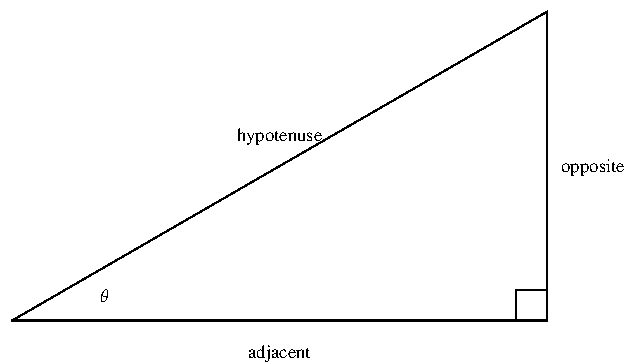
\includegraphics[width=5cm]{trigonometry/pictures/app-d-ratiosa.pdf}%
}
&%
\multicolumn{2}{|c|}{%

\psset{xunit=1cm,yunit=1cm}
\begin{pspicture}(-4,-0.5)(1,4)
\psaxes[labels=none, ticks=none]{<->}(0,0)(-4,-0.5)(1,4)
\pscircle*(-3,2){0.07}
\psline(0,0)(-3,2)
\psarc[linecolor=red](0,0){0.5}{0}{146.3099}
\rput[br](-3.1, 2){$(x,y)$}
\rput[l](0.1, 0.7){$\theta$}
\rput[lb](-1.55, 1.1){$r$}
\psline[linestyle=dotted](-3, 2)(-3, 0)
\psline[linestyle=dotted](-3, 2)(0, 2)
\psline(-2.7, 0)(-2.7, 0.3)(-3, 0.3)
\psline(0, 1.7)(-0.3, 1.7)(-0.3, 2)
\end{pspicture}
%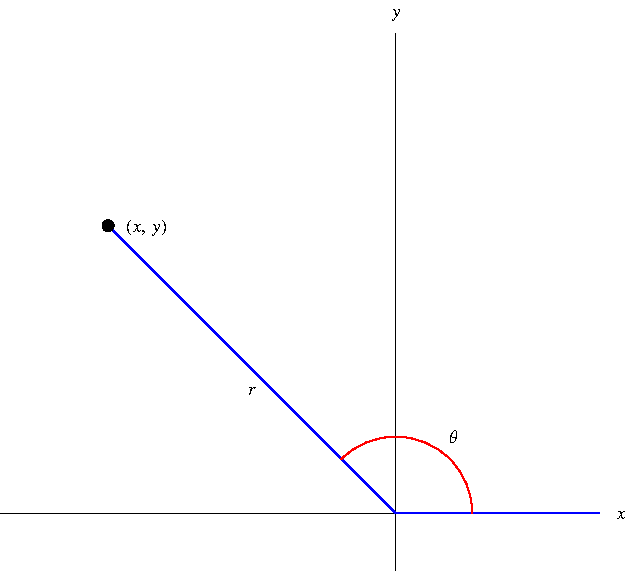
\includegraphics[width=5cm]{trigonometry/pictures/app-d-ratiosb.pdf}%
}\\%
\sin \theta = \frac{\textrm{opp}}{\textrm{hyp}} &
\csc \theta = \frac{\textrm{hyp}}{\textrm{opp}} &
\sin \theta = \frac{ y}{ r} &
\csc \theta = \frac{ r}{ y} \\
\cos \theta = \frac{\textrm{adj}}{\textrm{hyp}} &
\sec \theta = \frac{\textrm{hyp}}{\textrm{adj}} &
\cos \theta = \frac{ x}{ r} &
\sec \theta = \frac{ r}{ x} \\
\tan \theta = \frac{\textrm{opp}}{\textrm{adj}} &
\cot \theta = \frac{\textrm{adj}}{\textrm{opp}} &
\tan \theta = \frac{ y}{ x} &
\cot \theta = \frac{ x}{ y} \\
\hline
\multicolumn{2}{|c|}{\textrm{Acute angles}}&
\multicolumn{2}{|c|}{\textrm{Obtuse or negative angles}}\\
\hline
\end{array}
\]
\end{frame}
% end module trig-functions